%
% 2d.tex
%
% (c) 2018 Prof Dr Andreas Müller, Hochschule Rapperswil
%
\section{Inkompressible zweidimensionale Strömung}
\rhead{Inkompressible zweidimensionale Strömung}
Die Kontinuitätsgleichung
und die Navier-Stokes-Gleichung gelten auch für eine zweidimensionale
Strömung.
Im allgmeinen Fall ist die Strömung in zwei Dimensionen nicht wesentlich
leichter zu berechnen.
Nur im Falle einer inkompressiblen Strömung oder der Boussinesq-Approximation
spielt die Dichte in den Gleichungen keine Rolle, was erlaubt,
sie weiter zu vereinfachen:
\begin{align}
0
&=
-\nabla\cdot\vec v
\label{skript:2dim kontinuitaet}
\\
\frac{\partial \vec{v}}{\partial t}
&=
-\nabla\cdot(\vec{v}\vec{v})+\vec b + \frac1{\varrho}\nabla\cdot\bm{\tau}.
\label{skript:2dim navier-stokes}
\end{align}
Im Falle der Boussinesq-Approximation kommt auf der rechten Seite noch
ein Term für die Auftriebskraft hinzu.

Die Gleichungen
\eqref{skript:2dim kontinuitaet}
und
\eqref{skript:2dim navier-stokes}
bilden ein System von partiellen Differentialgleichungen für die zwei
unbekannten Funktionen $v_x$ und $v_y$, die Komponenten der 
Strömungsgeschwindigkeit.
Wir werden im Folgenden zeigen, dass die 
Gleichung~\eqref{skript:2dim kontinuitaet}
ermöglicht, das System auf eine einzelne partielle Differentialgleichung
für nur eine einzige Funktion zu reduzieren.

\subsection{Satz von Green}
\begin{figure}
\centering
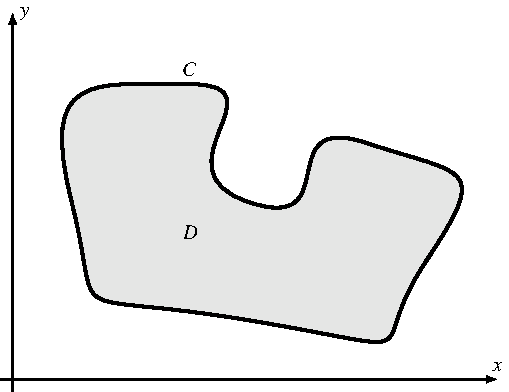
\includegraphics{chapters/2/green-curve.pdf}
\caption{Satz von Green: Das Wegintegral entlang der Randkurve $C$
stimmt mit dem zweifachen Integral über $D$ überein.
\label{skript:green-kurve}}
\end{figure}
Die Kontinuitätsgleichung 
\eqref{skript:2dim kontinuitaet}
ist ausgeschrieben
\[
0
=
\nabla\cdot\vec v
=
\frac{\partial v_x}{\partial x} + \frac{\partial v_y}{\partial y}.
\]
Die Divergenz auf der rechten Seite kommt auch im Satz von Green
vor:

\begin{satz}[Green]
\label{skript:2dim green}
Sei $D$ in kompaktes Gebiet in der $x$-$y$-Ebene mit Rand $\partial D=C$.
Weiter seien $f,g\colon D\to\mathbb R$ stetige Funktionen, die in $D$ 
stetig differenzierbar sind.
Dann gilt
\begin{equation}
\iint_{D}
\frac{\partial g(x,y)}{\partial x}
-
\frac{\partial f(x,y)}{\partial y}\,dx\,dy
=
\oint_C (f(x,y)\,dx + g(x,y)\,dy)
\label{skript:green formel}
\end{equation}
(Abbildung~\ref{skript:green-kurve}).
\end{satz}

\begin{figure}
\centering
\subfigure{}{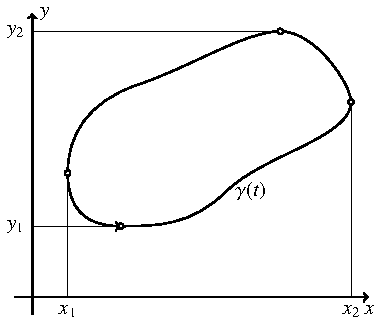
\includegraphics{chapters/2/pfadc.pdf}}
\subfigure{}{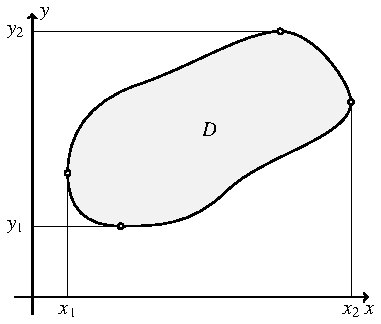
\includegraphics{chapters/2/pfad.pdf}}
\caption{Pfad $\gamma(t)$ in der $x$-$y$-Ebene und das vom Pfad eingeschlossen
Gebiet $D$.
\label{green:beweis}}
\end{figure}

Das Integral auf der rechten Seite wird mit Hilfe einer Parametrisierung
$\gamma\colon [a,b]\to\mathbb R^2$ der Randkurve $C$ definiert:
\begin{align*}
\oint_C f(x,y)\,dx
&=
\int_a^b f(\gamma_x(t),\gamma_y(t))\,\dot{\gamma}_x(t)\,dt
%\\
&&\text{und}&
\oint_C g(x,y)\,dy
&=
\int_a^b g(\gamma_x(t),\gamma_y(t))\,\dot{\gamma}_y(t)\,dt.
\end{align*}
Es kann auch vektoriell mit dem Skalarprodukt als
\[
\oint_C
\underbrace{
\begin{pmatrix}f\\g\end{pmatrix}
}_{\displaystyle =\vec{w}}
\cdot
\begin{pmatrix}\dot\gamma_x\\\dot\gamma_y\end{pmatrix}
\,dt
=
\oint_C \vec{w}\cdot\dot\gamma(t)\,dt
=:
\oint_C \vec{w}\cdot d\vec{s}
\]
geschrieben werden kann.
Der Weg $\gamma$ und das Gebiet $D$ ist in Abbildung~\ref{green:beweis}
dargestellt.

\begin{figure}
\centering
\subfigure{}{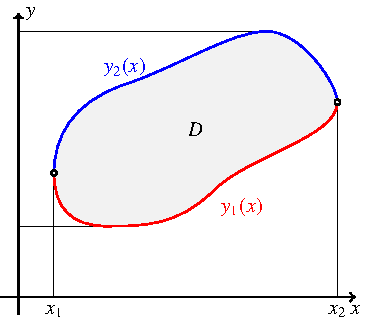
\includegraphics{chapters/2/pfadx.pdf}}
\subfigure{}{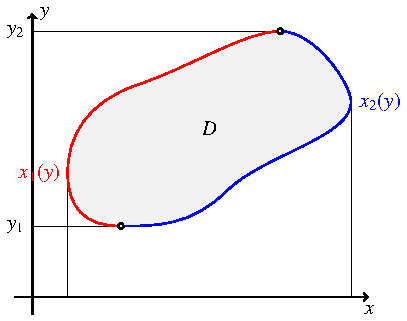
\includegraphics{chapters/2/pfady.pdf}}
\caption{Das Gebiet $D$ kann einerseits durch die Funktionen
$y_1(x)$ und $y_2(x)$ in Abhängigkeit von $x$ beschreiben werden,
andererseits kann es durch die Funktionen
$x_1(y)$ und $x_2(y)$ in Abhängigkeit von $y$ beschreiben werden.
\label{green:zweiraender}}
\end{figure}


\begin{proof}[Beweis]
Wir berechnen das Integral \label{skript:green formel}
über $D$ für jeden Summanden des Integranden einzeln, wobei
wir für die Beschreibung des Randes die Funktionen $y_i(x)$ und
$x_i(y)$ wie in Abbildungen~\ref{green:zweiraender} verwenden.

Das Integral über den ersten Summanden ist
\begin{align*}
\int_D
-\frac{\partial f(x,y)}{\partial y}
\,dx\,dy
&=
\int_{x_1}^{x_2}
\int_{y_1(\xi)}^{y_2(\xi)}
-\frac{\partial f(x,y)}{\partial y}
\,d\eta\,d\xi
=
\int_{x_1}^{x_2}
\biggl[
-f(\xi,\eta)
\biggr]_{y_1(\si)}^{y_2(\xi)}
\,d\xi
\\
&=
\int_{x_1}^{x_2} f(\xi,y_1(\xi))\,d\xi
-
\int_{x_1}^{x_2} f(\xi,y_2(\xi))\,d\xi.
\\
&=
\oint_\gamma f(x,y)\,dx.
\\
\intertext{Analog finden wir}
\int_D
\frac{\partial g(x,y)}{\partial x}
\,dx\,dy
&=
\int_{y_1}^{y_2}
\int_{x_1(\eta)}^{x_2(\eta)}
\frac{\partial g(\xi,\eta)}{\partial x}
\,d\xi
\,d\eta
\\
&=
\int_{y_1}^{y_2}
g(x_2(\eta),\eta) - g(x_1(\eta),\eta)
\,d\eta
\\
&=
\oint_\gamma g(x,y)\,dy.
\end{align*}
Zusammen ergeben diese
\[
\int_D
\frac{\partial g(x,y)}{\partial x}
-
\frac{\partial f(x,y)}{\partial y}
\,dx\,dy
=
\oint_\gamma
(
f(x,y)\,dx
+
g(x,y)\,dy
).
\]
Damit ist der Satz von Green bewiesen.
\end{proof}

\begin{satz}
\label{skript:wegunabhaengigkeit}
Das Wegintegral 
\[
\int_{\gamma}(f(x,y)\,dx + g(x,y)\,dy)
\]
ist genau dann unabhängig von der Wahl des Weges zwischen zwei
festen Punkten $P_0=(x_0,y_0)$ und $P_1=(x_1,y_1)$, wenn gilt
\[
0
=
\frac{\partial g(x,y)}{\partial x}-\frac{\partial f(x,y)}{\partial y}
=
\nabla\cdot
\begin{pmatrix}-g(x,y)\\\phantom{-}f(x,y)\end{pmatrix}.
\]
\end{satz}

\begin{proof}[Beweis]
Sind $\gamma_1$ und $\gamma_2$ zwei verschiedene Wege von $P_0$ nach
$P_1$, dann kann man einen geschlossenen Weg $\gamma$ von $P_0$ nach
$P_0$ konstruieren indem man zuerst den Weg $\gamma_1$ durchläuft und
anschliessend den Weg $\gamma_2$ in umgekehrter Richtung.
Das Wegintegral über den Weg $\gamma$ ist
\begin{align}
\oint_{\gamma}(f(x,y)\,dx + g(x,y)\,dy)
&=
\int_{\gamma_1} (f(x,y)\,dx + g(x,y)\,dy)
-
\int_{\gamma_2} (f(x,y)\,dx + g(x,y)\,dy).
\label{green:integrale}
\intertext{%
Sei $D$ das Gebiet, das von $\gamma$ berandet wird,
dann gilt nach dem Satz von Green andererseits
}
&=
\int_D
\frac{\partial g(x,y)}{\partial x}-\frac{\partial f(x,y)}{\partial y}
\,dx\,dy
=0.
\end{align}
Die beiden Integrale in~\eqref{green:integrale} müssen also übereinstimmen.

Sei umgekehrt das Wegintegral zwischen zwei Punkten immer unabhängig
vom Weg zwischen den Punkten.
Dann betrachten wir die Wegintegrale zwischen den Ecken
$(x,y)$ und $(x+\Delta x,y+\Delta y)$ eines Rechtecks $R$.
Der eine Weg folgt zuerst der unteren Kante des Rechtecks und dann
der rechten, der andere Weg folgt erst der linken Kante und dann der
oberen.
Die beiden Wegintegrale sind gleich, also verschwindet das Wegintegral
über den Rand des Rechtecks $R$.
Das Wegintegral über den Rand $\partial R$ von $R$ ist
\begin{align*}
0
&=
\int_{\partial R} (f(x,y)\,dx + g(x,y)\,dy)
\\
&=
f(x,y)\Delta x
+ g(x+\Delta x,y) \Delta y
- f(x,y+\Delta y) \Delta x
- g(x,y) \Delta y
+ o(\Delta x\,\Delta y)
\\
&=
\biggl(
\frac{f(x,y)-f(x,y+\Delta y)}{\Delta y}
+
\frac{g(x+\Delta x,y)-g(x,y)}{\Delta }
\biggr)
\Delta x\,\Delta y
+ o(\Delta x\,\Delta y)
\end{align*}
Dies funktioniert nur, wenn der Klammerterm im Grenzwert $\Delta x\to 0$ und
$\Delta y\to 0$ verschwindet, also
\[
-
\frac{\partial f(x,y)}{\partial y}
+
\frac{\partial g(x,y)}{\partial x}
=0,
\]
wie im Satz behauptet.
\end{proof}


\subsection{Stromfunktion}
Wir wenden den Satz \ref{skript:2dim green} von Green auf die
Funktionen $f(x,y)=-v_y(x,y)$ und $g(x,y)=v_x(x,y)$ an.
Die Formel \eqref{skript:green formel} ergibt
\begin{equation}
\oint_C (-v_y(x,y)\,dx + v_x(x,y)\,dy)
=
\iint_D
\underbrace{
\frac{\partial v_x(x,y)}{\partial x}
+
\frac{\partial v_y(x,y)}{\partial y}
}_{\displaystyle=0}
\,dx\,dy
=
0.
\label{skript:wegunabh}
\end{equation}
Man kann dieses Resultat auch wie folgt interpretieren.
Wenn $C_1$ und $C_2$ zwei Kurven sind, die den Punkt $A$ mit dem Punkt $B$
verbinden, dann lässt sich eine geschlossene Kurve $C$ konstruieren, indem
zuerst die Kurve $C_1$ von $A$ nach $B$ durchlaufen wird und dann die
Kurve $C_2$ in umgekehrter Richtung von $B$ nach $A$.
Die Formel \eqref{skript:wegunabh} besagt dann, dass 
\begin{align*}
0
&=
\oint_{C} (-v_y(x,y)\,dx + v_x(x,y)\,dy)
\\
&=
\int_{C_1} (-v_y(x,y)\,dx + v_x(x,y)\,dy)
-
\int_{C_2} (-v_y(x,y)\,dx + v_x(x,y)\,dy)
\end{align*}
oder
\begin{align*}
\Rightarrow
\qquad
\int_{C_1} (-v_y(x,y)\,dx + v_x(x,y)\,dy)
&=
\int_{C_2} (-v_y(x,y)\,dx + v_x(x,y)\,dy).
\end{align*}
Das Wegintegral hängt also nicht von der Wahl des Weges ab, jeder Weg
von $A$ nach $B$ führt auf den gleichen Wert des Integrals.

\begin{figure}
\centering
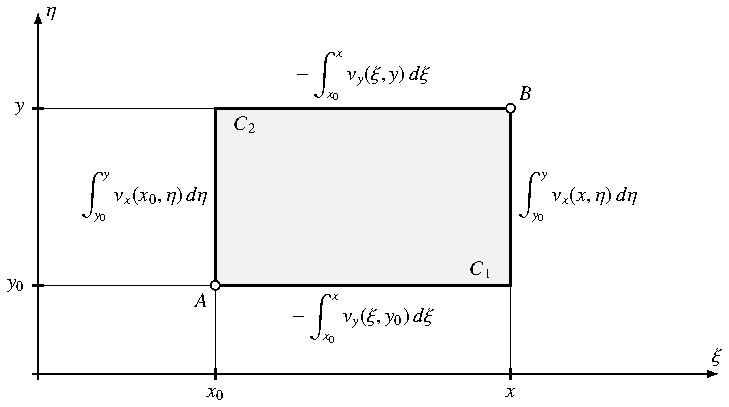
\includegraphics{chapters/2/green-curves.pdf}
\caption{Verschiedene Pfade zur Berechnung der Funktion $\psi(B)$
führen auf den gleichen Wert von $\psi(B)$ und ermöglichen, die partiellen
Ableitungen zu berechnent.
\label{skript:psi-pfade}}
\end{figure}

Wir halten den Punkt $A$ fest und definieren die Funktion
\[
\psi(B)
=
\int_C (-v_y(x,y)\,dx + v_x(x,y)\,dy)
\]
für einen beliebigen Weg von $A$ nach $B$. 
Zum Beispiel können für die Berechnung die Kurven
$C_1$ oder $C_2$ in Abbildung~\ref{skript:psi-pfade}
verwendet werden.
Damit lassen sich die Integrale ausschreiben:
\begin{align*}
\psi(x,y)
&=
\int_{C_1} (-v_y(x,y)\,dx + v_x(x,y)\,dy)
=
-\int_{x_0}^x v_y(\xi, y_0)\,d\xi
+
\int_{y_0}^y v_x(x,\eta)\,d\eta
\\
&=
\int_{C_2} (-v_y(x,y)\,dx + v_x(x,y)\,dy)
=
\int_{y_0}^y v_x(x_0,\eta)\,d\eta
-
\int_{x_0}^x v_y(\xi,y)\,d\xi.
\end{align*}
Diese Ausdrücke erlauben uns, die partiellen Ableitungen von $\psi(x,y)$
zu berechnen.
Für die Ableitung nach $x$ verwenden wir den zweiten Ausdruck, für die
Ableitung nach $y$ den ersten.
Wir erhalten
\begin{align*}
\frac{\partial\psi(x,y)}{\partial x}
&=
-\frac{\partial}{\partial x} \int_{x_0}^x v_y(\xi,y)\,d\xi
=
-v_y(x,y)
%\\
&&\text{und}&
\frac{\partial\psi(x,y)}{\partial y}
&=
\frac{\partial}{\partial y} \int_{y_0}^y v_x(x,\eta)\,d\eta
=
v_x(x,y).
\end{align*}
In vektorieller Form kann man dies auch als
\begin{equation}
\vec{v}
=
\begin{pmatrix}v_x\\v_y \end{pmatrix}
=
\underbrace{
\begin{pmatrix}0&-1\\1&0\end{pmatrix}
}_{\displaystyle=J}
\begin{pmatrix}
\frac{\partial\psi}{\partial x}\\
\frac{\partial\psi}{\partial y}
\end{pmatrix}
=
J\nabla\psi
\label{skript:Jnablapsi}
\end{equation}
schreiben.
Aus der Funktion $\psi$ lässt sich das Vektorfeld $\vec{v}$ also wieder
rekonstruieren.
Sie heisst die {\em Stromfunktion} des Vektorfeldes $\vec{v}$.
\index{Stromfunktion}%
Natürlich ist $\psi(x,y)$ nur bis auf eine Konstante bestimmt.

Umgekehrt ist für jede beliebige Funktion $\varphi(x,y)$ das Vektorfeld
$\vec{u}=J\nabla\varphi$ divergenzfrei:
\begin{align*}
\nabla\cdot\vec{u}
=
\frac{\partial}{\partial x}
\biggl(-\frac{\partial\varphi}{\partial y}\biggr)
+
\frac{\partial}{\partial y}
\biggl(\frac{\partial\varphi}{\partial x}\biggr)
=
-\frac{\partial^2\varphi}{\partial x\,\partial y}
+\frac{\partial^2\varphi}{\partial y\,\partial x}
=
0.
\end{align*}
Die Darstellung \eqref{skript:Jnablapsi} des Geschwindigkeitsfeldes 
erlaubt eine geometrische Interpretation.
Der Gradient $\nabla\psi$ ist ein Vektorfeld, welches auf den
Niveaulinien der Funktion $\psi$ senkrecht steht.
Je schneller die Zunahme von $\psi$, desto grösser ist der
Vektor $\nabla\psi$.

Die Matrix $J$ ist eine Drehmatrix, sie dreht Vektoren um $90^\circ$ 
im Gegenuhrzeigersinn.
Die Vektoren $J\nabla\psi$ sind also tangential an die Niveaulinien,
die Niveaulinien sind gleichzeitig die Stromlinien der Strömung.
Ist die Strömung auf ein kompaktes Gebiet beschränkt, dann ist der
Rand des Gebietes eine Stromlinie, also eine Niveaulinie von $\psi$.
Da $\psi$ nur bis auf eine Konstante festgelegt ist, kann man $\psi$
so wählen, dass der Rand des Gebietes durch die Gleichung $\psi(x,y)=0$
beschrieben wird.

\index{Stromlinien}
\begin{figure}
\centering
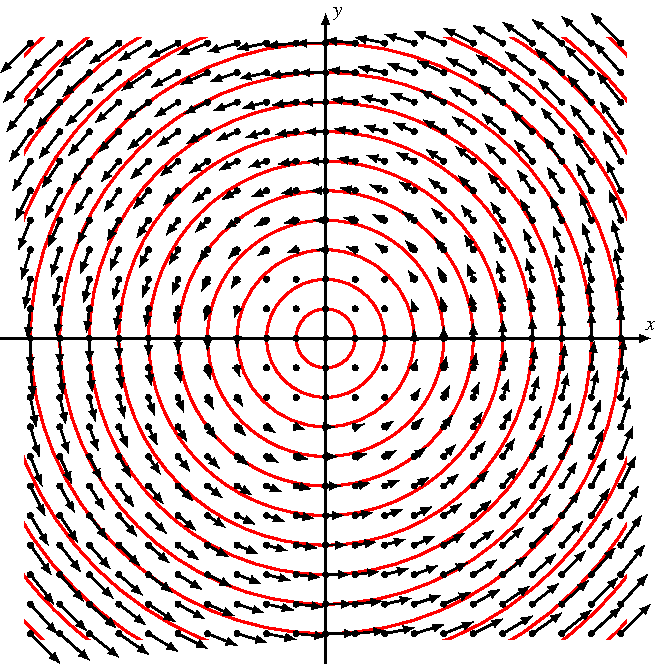
\includegraphics{chapters/2/rotation.pdf}
\caption{Strömungsfunktion $\psi(x,y)=a(x^2+y^2)$ und das zugehörige
Vektorfeld.
Die Strömungsgeschwindigkeit ist proportional zum Radius, es handelt
sich also um eine starre Drehung um den Nullpunkt.
\label{skript:rotation}}
\end{figure}
\begin{beispiel}
Die Funktion $\psi(x,y)=a(x^2+y^2)$ führt auf das Vektorfeld
\[
\vec{v}
=
J\nabla\psi
=
2a
\begin{pmatrix}
-y\\x
\end{pmatrix}
\]
(Abbildung~\ref{skript:rotation}).
Die Strömungsgeschwindigkeit ist $2a\sqrt{x^2+y^2}=2ar$, es handelt sich
also um eine starre Drehung um den Nullpunkt des Koordinatensystems mit
Winkelgeschwindigkeit $\omega=2a$.
\end{beispiel}

\subsection{Vorticity}
Wir suchen eine Grösse, mit der wir das Ausmass messen können, wie schnell
sich das Fluid dreht.
Die Winkelgeschwindigkeit bei der Drehung um den Punkt $(x,y)$ können wir
durch Vergleich der Geschwindigkeit an den Punkten $(x\pm h,y)$ und
$(x,y\pm h)$ finden.
Es ist
\[
\omega
=
\frac{v_y(x+h),y) - v_y(x-h,y)}{2h}
=
\frac{-v_x(x,y+h) + v_x(x,y-h)}{2h}.
\]
Beim Grenzübergang $h\to 0$ erhalten wir
\[
\omega
=
\frac{\partial v_y(x,y)}{\partial x}
=
-\frac{\partial v_x{x,y}}{\partial y}
\qquad\text{oder}\qquad
2\omega
=
\frac{\partial v_y}{\partial x}-\frac{\partial v_x}{\partial y}.
\]
Damit haben wir eine Grösse gefunden, die als Mass für die Drehgeschwindigkeit
dienen kann.
\index{Vorticity}
\begin{definition}
Ist $\vec{v}$ das Geschwindigkeitsfeld der Strömung, dann schreiben wir
\[
\nabla\times\vec{v}
=
\frac{\partial v_y}{\partial x}-\frac{\partial v_x}{\partial y}
=
\zeta.
\]
Die Funktion $\zeta$ heisst die {\em Vorticity} des Strömungsfeldes.
\end{definition}

Beschreibt man die Strömung mit Hilfe der Strömungsfunktion, dann gilt
für die Vorticity
\begin{equation}
\zeta
=
\nabla\times\vec{v}
=
\nabla\times J\nabla\psi
=
\frac{\partial}{\partial x}
\biggl(-\frac{\partial\psi}{\partial y}\biggr)
-
\frac{\partial}{\partial x}
\frac{\partial\psi}{\partial x}
=
-\biggl(
\frac{\partial^2\psi}{\partial x^2}
+
\frac{\partial^2\psi}{\partial y^2}
\biggr)
=
-\Delta \psi.
\label{skript:stroemung-vorticity}
\end{equation}
Der Laplace-Operator verbindet also die Strömungsfunktion direkt mit der
Vorticity.
Für die Strömung in einem kompakten Gebiet $\Omega$ ist der Rand eine
Niveaulinie von $\psi$.
Wie früher dargelegt können wir $\psi$ so wählen, dass $\psi=0$ gilt auf
dem Rand.
Bei gegebener Vorticity $\zeta$ ist daher $\psi$ die Lösung der
partiellen Differentialgleichung
\begin{equation}
\Delta \psi = -\zeta\quad\text{in $\Omega$}
\qquad
\text{und}
\qquad
\psi = 0\quad\text{auf $\partial\Omega$}.
\label{skript:zetapsielliptisch}
\end{equation}
Die Theorie der elliptischen partiellen Differentialgleichungen 
sagt, dass $\psi$ eindeutig bestimmt ist.
Statt die Strömungsgleichungen für $\psi$ zu lösen, können wir
also auch versuchen, eine Gleichung für die Vorticity $\zeta$
aufzustellen und dann mit Hilfe des elliptischen partiellen
Randwertproblems \eqref{skript:zetapsielliptisch} die Strömungsfunktion
$\psi$
und schliesslich $\vec{v}$ bestimmen.

Um die Differentialgleichung für $\zeta$ zu finden, wenden wir den
Operator $\nabla\times\mathstrut$ auf die Bewegungsgleichung
\eqref{skript:2dim navier-stokes}
an:
\[
\nabla\times\frac{\partial \vec{v}}{\partial t}
=
-\nabla\times(\nabla\cdot(\vec{v}\vec{v}))+\nabla\times\vec b + \nabla\times\biggl(\frac1{\varrho}\nabla\cdot\bm{\tau}\biggr).
\]
Die linke Seite ist die Zeitableitung der Vorticity.
Die Divergenz von $\vec{v}\vec{v}$ ist 
\[
(\nabla\cdot(\vec{v}\vec{v}))_j
=
\sum_i \frac{\partial}{\partial i}v_iv_j
=
\biggl(\sum_i \frac{\partial v_i}{\partial i}\biggr)v_j
+
\sum_i v_i\frac{\partial v_j}{\partial i}
=
(\underbrace{\nabla\cdot\vec{v}}_{\displaystyle=0})v_j
+
\vec{v}\cdot\nabla v_j.
\]
Es folgt
\[
\nabla\cdot(\vec{v}\vec{v})
=
\vec{v}\cdot\nabla \vec{v}.
\]
Daraus kann man jetzt auch die Vorticity berechnen:
\begin{align*}
\nabla\times(\nabla\cdot(\vec{v}\vec{v}))
&=
\nabla\times(\vec{v}\cdot\nabla\vec{v})
=
\frac{\partial}{\partial x}(\vec{v}\cdot\nabla v_y)
-
\frac{\partial}{\partial y}(\vec{v}\cdot\nabla v_x)
\\
&=
\vec{v}\cdot\nabla
\biggl(\frac{\partial v_y}{\partial x}-\frac{\partial v_x}{\partial y}\biggr)
+
\frac{\partial\vec{v}}{\partial x} \cdot\nabla v_y
-
\frac{\partial\vec{v}}{\partial y} \cdot\nabla v_x
\\
&=
\vec{v}\cdot\nabla\zeta
+
\frac{\partial v_x}{\partial x} \frac{\partial v_y}{\partial x}
+
\frac{\partial v_y}{\partial x} \frac{\partial v_y}{\partial y}
-
\frac{\partial v_x}{\partial y} \frac{\partial v_x}{\partial x}
-
\frac{\partial v_y}{\partial y} \frac{\partial v_x}{\partial y}
\\
&=
\vec{v}\cdot\nabla\zeta
+
\frac{\partial v_x}{\partial x}
\biggl(\frac{\partial v_y}{\partial x}-\frac{\partial v_x}{\partial y}\biggr)
+
\frac{\partial v_y}{\partial y}
\biggl(\frac{\partial v_y}{\partial x}-\frac{\partial v_x}{\partial y}\biggr)
\\
&=
\vec{v}\cdot\nabla\zeta
+
(\nabla\cdot\vec{v})\zeta
=
\vec{v}\cdot\nabla\zeta.
\end{align*}
Wir waren also nicht ganz erfolgreich, die Geschwindigkeit aus der
Bewegungsgleichung zu eliminieren.
Wir haben nur die Form
\[
\frac{\partial \zeta}{\partial t}
=
-\vec{v}\cdot\nabla\zeta
+\nabla\times\vec b
+ \nabla\times\biggl(\frac1{\varrho}\nabla\cdot\bm{\tau}\biggr)
\]
erreicht.
Ausserdem ist es möglich, dass die Spannungen $\bm{\tau}$ ebenfalls von
den Geschwindigkeiten abhängig sind.

Wir können aber die Vorticity auch noch durch die Strömungsfunktion
ausdrücken.
Ersetzen wir $\zeta=-\Delta\psi$ in der Bewegungsgleichung, erhalten
wir
\begin{equation}
\frac{\partial \Delta \psi}{\partial t}
=
-J\nabla\psi\cdot\nabla\Delta\psi
+\nabla\times\vec b
+ \nabla\times\biggl(\frac1{\varrho}\nabla\cdot\bm{\tau}\biggr).
\label{skript:voritictyequation}
\end{equation}
Jetzt ist die Strömung vollständig durch die einzige unbekannte Funktion 
$\psi$ beschrieben.

Der erste Term auf der rechten Seite von \eqref{skript:voritictyequation}
kann noch etwas kompakter geschrieben werden.
Es ist
\begin{align*}
(J\nabla f)\cdot(\nabla g)
&=
\begin{pmatrix}
-\frac{\partial f}{\partial y}
\\
\frac{\partial f}{\partial x}
\end{pmatrix}
\cdot
\begin{pmatrix}
\frac{\partial g}{\partial x}\\
\frac{\partial g}{\partial y}
\end{pmatrix}
=
\frac{\partial f}{\partial x}
\frac{\partial g}{\partial y}
-\frac{\partial f}{\partial y}
\frac{\partial g}{\partial x}.
\end{align*}
Der Ausdruck auf der rechten Seite kommt auch in anderem Zusammenhang vor.

\begin{definition}
Seien $f$ und $g$ Funktionen der Variablen $x$ und $y$.
Dann heisst
\[
\frac{\partial(f,g)}{\partial(x,y)}
=
\frac{\partial f}{\partial x}
\frac{\partial g}{\partial y}
-
\frac{\partial f}{\partial y}
\frac{\partial g}{\partial x}
\]
die
{\em Funktionaldeterminante} oder {\em Jacobische Determinante} von
$f$ und $g$.
\end{definition}
\index{Funktionaldeterminante}%
\index{Jacobi-Determinante}%
Mit dieser Definition wird die Bewegungsgleichung
\begin{equation}
\frac{\partial \Delta \psi}{\partial t}
=
\nabla\times\vec b
+ \nabla\times\biggl(\frac1{\varrho}\nabla\cdot\bm{\tau}\biggr)
-\frac{\partial(\psi,\Delta\psi)}{\partial(x,y)}.
\label{skript:psidgl}
\end{equation}
Im Falle der Boussinesq-Näherung kommt noch ein Term für den
Auftrieb hinzu.

\subsection{Spannungen und Stromfunktion}
Für eine newtonsche Flüssigkeit haben wir in 
\eqref{skript:inkompressibel newtonsch}
bereits den Spannungstensor durch den Druck und die Spannungen
ausgedrückt.
Aus der Bewegungsgleichung für die Geschwindigkeit haben wir die
Differentialgleichung \eqref{skript:psidgl} erhalten, indem
wir den Operator $\nabla\times\mathstrut$ angewendet haben.
Wir müssen jetzt also 
\[
\nabla\times\biggl(\frac1{\varrho}(\nabla p-\nu\Delta\vec{v})\biggr)
=
\frac{1}{\varrho}
\biggl(
\nabla\times\nabla p
-
\nu \nabla\times\Delta\vec{v}
\biggr)
=
\frac1{\varrho}
\biggl(
\frac{\partial}{\partial x}\frac{\partial p}{\partial y}
-
\frac{\partial}{\partial y}\frac{\partial p}{\partial x}
-\nu\Delta\nabla\times\vec{v}
\biggr)
\]
berechnen.
Der erste Term fällt weg, weil es auf die Reihenfolge der
Ableitungen nicht ankommt.
Im letzten Term haben wir angenommen, dass $\nu$ nicht vom Ort
abhängt.
Dies ist genau genommen nicht richtig, da $\nu$ zum Beispiel
stark von der Temperatur abhängt, die ebenfalls nicht konstant sein
muss.
Der zweite Term in der Klammer ist natürlich einfach
$\nu\Delta\zeta=-\nu\Delta^2\psi$.
Damit bekommen wir die Bewegungsgleichung für $\psi$ in der Form
\begin{equation}
\frac{\partial \Delta \psi}{\partial t}
=
\nabla\times\vec b
+\frac{\nu}{\varrho}\Delta^2\psi
-\frac{\partial(\psi,\Delta\psi)}{\partial(x,y)}.
\label{skript:psidgl2}
\end{equation}

